% Schéma pevného disku: plotny na společném vřetenu, stopy a sektory,
% cylindr a sestava ramének s hlavami nad i pod každou plotnou.
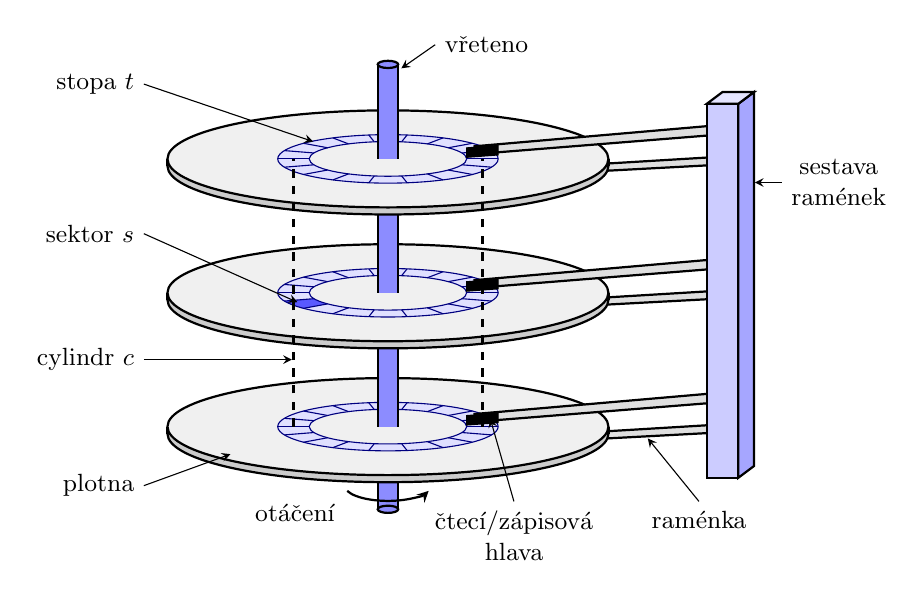
\begin{tikzpicture}[
    x=1cm, y=1cm,
    >=stealth,
    every node/.style={font=\small},
    lab/.style={font=\small, align=center},
    callout/.style={->, thin}
]

    % Parametry: poměr zploštění elips (pohled šikmo shora),
    % poloměr plotny, vnitřní a vnější poloměr zvýrazněné stopy
    \def\hddys{0.22}
    \def\hddR{2.8}
    \def\hddti{1.0}
    \def\hddto{1.4}
    \def\hddtm{1.2}
    \def\hddspw{0.13}

    \colorlet{spindlecol}{blue!45}
    \colorlet{armcol}{gray!25}

    % Spodní konec vřetena
    \fill[spindlecol] (-\hddspw,-2.75) rectangle (\hddspw,-1.7);
    \draw[thick] (-\hddspw,-2.75) -- (-\hddspw,-1.7) (\hddspw,-2.75) -- (\hddspw,-1.7);
    \draw[thick, fill=spindlecol] (0,-2.75) ellipse ({\hddspw} and {\hddspw*\hddys*1.6});

    \foreach \hddp/\sptop [count=\hddk] in {-1.7/0, 0/1.7, 1.7/2.9}{

        % Spodní raménko (pod plotnou, z velké části zakryté)
        \draw[thick, fill=armcol]
            (\hddtm-0.1,\hddp-0.16) -- (4.1,\hddp+0.02) -- (4.1,\hddp-0.08) -- (\hddtm-0.1,\hddp-0.24) -- cycle;

        % Plotna: hrana a horní plocha
        \draw[thick, fill=gray!40] (0,\hddp-0.09) ellipse ({\hddR} and {\hddR*\hddys});
        \fill[gray!40] (-\hddR,\hddp-0.09) rectangle (\hddR,\hddp);
        \draw[thick] (-\hddR,\hddp-0.09) -- (-\hddR,\hddp) (\hddR,\hddp-0.09) -- (\hddR,\hddp);
        \draw[thick, fill=gray!12] (0,\hddp) ellipse ({\hddR} and {\hddR*\hddys});

        \begin{scope}[shift={(0,\hddp)}, yscale=\hddys]
            % Zvýrazněná stopa rozdělená na sektory
            \fill[blue!12, even odd rule] (0,0) circle (\hddto) (0,0) circle (\hddti);
            \ifnum\hddk=2
                \fill[blue!65] (200:\hddti) arc (200:220:\hddti) -- (220:\hddto) arc (220:200:\hddto) -- cycle;
            \fi
            \draw[blue!50!black] (0,0) circle (\hddto) (0,0) circle (\hddti);
            \foreach \a in {0,20,...,340}{
                \draw[blue!50!black] (\a:\hddti) -- (\a:\hddto);
            }
        \end{scope}

        % Vřeteno nad plotnou
        \fill[spindlecol] (-\hddspw,\hddp) rectangle (\hddspw,\sptop);
        \draw[thick] (-\hddspw,\hddp) -- (-\hddspw,\sptop) (\hddspw,\hddp) -- (\hddspw,\sptop);

        % Horní raménko s čtecí/zápisovou hlavou nad stopou
        \draw[thick, fill=armcol]
            (\hddtm-0.1,\hddp+0.06) -- (4.1,\hddp+0.3) -- (4.1,\hddp+0.42) -- (\hddtm-0.1,\hddp+0.16) -- cycle;
        \draw[fill=black] (\hddtm-0.2,\hddp+0.02) -- (\hddtm+0.2,\hddp+0.05) -- (\hddtm+0.2,\hddp+0.17) -- (\hddtm-0.2,\hddp+0.14) -- cycle;
    }

    % Horní konec vřetena
    \draw[thick, fill=spindlecol] (0,2.9) ellipse ({\hddspw} and {\hddspw*\hddys*1.6});

    % Cylindr: stejné stopy na všech plotnách
    \draw[thick, dashed] (-\hddtm,-1.7) -- (-\hddtm,1.7);
    \draw[thick, dashed] (\hddtm,-1.7) -- (\hddtm,1.7);

    % Sestava ramének (aktuátor)
    \draw[thick, fill=blue!35] (4.45,-2.35) -- (4.65,-2.2) -- (4.65,2.55) -- (4.45,2.4) -- cycle;
    \draw[thick, fill=blue!20] (4.05,-2.35) rectangle (4.45,2.4);
    \draw[thick, fill=blue!10] (4.05,2.4) -- (4.25,2.55) -- (4.65,2.55) -- (4.45,2.4) -- cycle;

    % Otáčení
    \begin{scope}[shift={(0,-2.45)}, yscale=\hddys*1.6]
        \draw[->, thick] (200:0.55) arc (200:340:0.55);
    \end{scope}
    \node[lab, anchor=east] at (-0.55,-2.8) {otáčení};

    % =====================================================
    % Popisky
    % =====================================================
    \node[lab, anchor=west] (lspin) at (0.6,3.15) {vřeteno};
    \draw[callout] (lspin.west) -- (0.17,2.85);

    \node[lab, anchor=east] (ltrack) at (-3.1,2.65) {stopa $t$};
    \draw[callout] (ltrack.east) -- (-0.95,1.92);

    \node[lab, anchor=east] (lsect) at (-3.1,0.75) {sektor $s$};
    \draw[callout] (lsect.east) -- (-1.15,-0.12);

    \node[lab, anchor=east] (lcyl) at (-3.1,-0.85) {cylindr $c$};
    \draw[callout] (lcyl.east) -- (-1.22,-0.85);

    \node[lab, anchor=east] (lplat) at (-3.1,-2.45) {plotna};
    \draw[callout] (lplat.east) -- (-2.0,-2.05);

    \node[lab, anchor=north] (lhead) at (1.6,-2.65) {čtecí/zápisová\\hlava};
    \draw[callout] (lhead.north) -- (\hddtm+0.1,-1.6);

    \node[lab, anchor=north] (larm) at (3.95,-2.65) {raménka};
    \draw[callout] (larm.north) -- (3.3,-1.85);

    \node[lab, anchor=west] (lassy) at (5.0,1.4) {sestava\\ramének};
    \draw[callout] (lassy.west) -- (4.66,1.4);

\end{tikzpicture}
